\section{Simulated Dataset}\label{Dataset}\hfill

Jets and tracks measured by the ATLAS and CMS detectors are described using a 3D detector coordinate system with their transverse momentum, $p_{\rm T}$, and angular components, $\eta$, and $\phi$.\footnote{$\phi$ is azimuthal angle, $\eta=-\ln\left[ \tan\left( \frac{\theta}{2} \right) \right]$ where $\theta$ is polar angle, and $p_{\rm T}=|\overrightarrow{p}|\sin\theta$ in the spherical coordinate system where the $z$ axis is directed along the beam.}
%A clustering algorithm, such as anti-$k_t$~\cite{Cacciari_2008}, finds all possible sets of tracks within a certain cone of radius, $R$,\footnote{$R = \sqrt{( \eta_{jet} - \eta_{track})^2 + ( \phi_{jet} - \phi_{track})^2}$, where the $\phi$ difference is taken modulo $2\pi$.} greater than a minimum $p_{\rm T}$ threshold to form physics objects called jets.
Figure \ref{fig:HLLHC} depicts an unraveled view of the detector where jets, represented as circles, are sets of clustered tracks, represented as dots, with a minimum $p_{\rm T}$ requirement. As $\left\langle \mu \right\rangle$ increases, the pileup tracks form more jets, leading to a much higher number of jets per event at the same $p_{\rm T}$ as shown in \ref{fig:njets}. Jet features include: $[p_{\rm T},\eta,\phi,m]$, and track features include: $[p_{\rm T},\eta,\phi,m,d_0,z_0]$, where $d_0$ and $z_0$ are transverse and longitudinal distance to primary vertex when track is extrapolated to beam line using parameterized estimation described in~\cite{ATLAS:2021yvc}.

\begin{figure}[h]
\centering
\begin{subfigure}{.32\textwidth}
  \centering
  \textbf{\tiny{Event at $\left\langle \mu \right\rangle$=60}}
  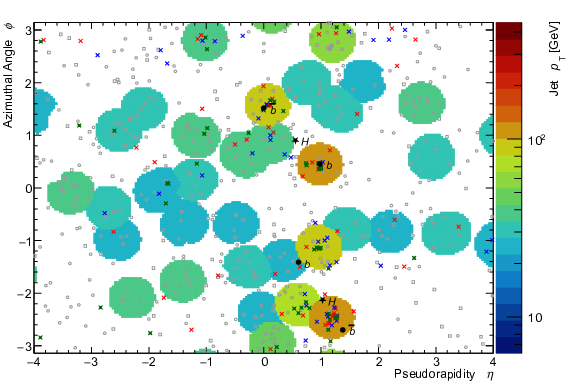
\includegraphics[width=1\textwidth]{Event_mu60.png}
  \caption{}
  \label{fig:sub1}
\end{subfigure}%
\begin{subfigure}{.32\textwidth}
  \centering
  \textbf{\tiny{Event at $\left\langle \mu \right\rangle$=200}}
  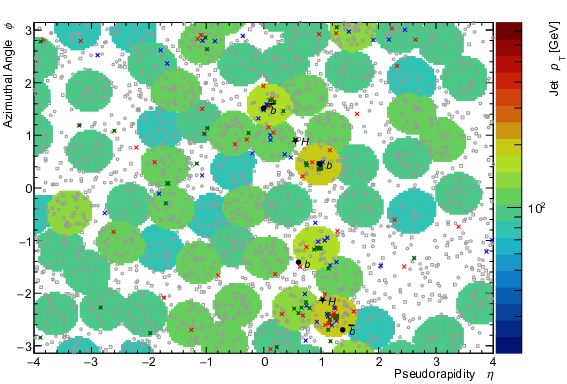
\includegraphics[width=1\linewidth]{Event_mu200.png}
  \caption{}
  \label{fig:sub2}
\end{subfigure}
\begin{subfigure}{.32\textwidth}
  %\textbf{\tiny{Dependence of Min Jet $p_{\rm T}$ on $\mu$}}
  \includegraphics[width=1\linewidth]{njet_vs_ptcut.png} 
  \caption{}
  \label{fig:njets}
\end{subfigure}

\caption{An example of an event at (a) $\left\langle \mu \right\rangle=60$ and (b) $\left<\mu\right>=200$. Jets are depicted as clusters of energy (large color circles). Pileup particles (small grey circles) at $\left\langle \mu \right\rangle=200$ begin to dominate the event and significantly distort the energy and mass of hard scatter jets. (c) As $\left\langle \mu \right\rangle$ increases, the minimum jet $p_{\rm T}$ parameter must increase to keep jets per event constant. }
\label{fig:HLLHC}
\end{figure}

To evaluate the performance of \myname{}, a specific physics process is chosen: the simultaneous production of two Higgs bosons decaying into a $b$-anti $b$ quark pair. This process is of high interest for HEP and is one of the key components for the HL-LHC physics program~\cite{Dainese:2019rgk}. Each Higgs boson gives rise to a pair of jets $\overrightarrow{J}_i$, $\overrightarrow{J}_j$, described by a combined 4-vector $\overrightarrow{J}_{ij}$. When paired through the proper combinatorics, the distribution of the $\overrightarrow{J}_{ij}$ mass forms a resonance peak near the expected Higgs mass, $m_{\rm H}\approx125$~GeV, but pileup contamination will shift and widen the peak.

%\begin{figure}[h]
%\centering
%  \includegraphics[width=0.6\linewidth+]{figures/njet_vs_ptcut.png} 
%  \caption{The simulated average number of jets per event as a function of minimum jet $p_{\rm T}$ at $\left\langle \mu \right\rangle=60$ for the LHC and $\left\langle \mu \right\rangle=200$ for the HL-LHC for the $HH \rightarrow b\bar{b}b\bar{b}$ sample. In high pileup conditions, the dominant pileup background significantly inflates the momentum of all jets, leading to more jets per event for a given minimum jet momentum. }
%\label{fig:njets}
%\end{figure}

A sample of 50k di-Higgs events is generated using MadGraph interfaced with Pythia \footnote{The process \texttt{p p > h h, h > b b\~{}} generated with MadGraph5\_aMC@NLO v3.5.5~\cite{madgraph} interfaced to Pythia 8.312~\cite{pythia}.}. Samples are simulated at $\left\langle \mu \right\rangle = 60$ for the LHC pileup conditions and at $\left\langle \mu \right\rangle = 200$ for the HL-LHC pileup conditions. Pileup processes\footnote{The process \texttt{SoftQCD:inelastic} generated with Pythia using the A14 central tune~\cite{TheATLAScollaboration:2014rfk} and NNPDF2.3LO~\cite{BALL2013244}.} are overlaid according to a Poisson distribution with mean of $\left<\mu\right>$. The position of each hard scatter and pileup vertex in the event is independently smeared according to a Gaussian distribution with $\sigma_{x,y}=0.3$~mm in transverse plane and $\sigma_z=50$~mm along the direction of the proton beam to mimic the actual LHC conditions. Stable particles are then passed to FastJet~\cite{Cacciari_2012} to be clustered into jets using anti-$k_t$ algorithm~\cite{Cacciari_2008} with the cone size $R=0.4$ \footnote{$R = \sqrt{( \eta_{jet} - \eta_{track})^2 + ( \phi_{jet} - \phi_{track})^2}$, where the $\phi$ difference is taken modulo $2\pi$.} and minimum jet $p_{\rm T}$ of 25~GeV. To incorporate detector limitations, neutral particles and particles with $p_{\rm T}$ below 400~MeV are removed from the dataset.
